\section{Platforms}
\label{platforms}


Unless software is distributed on dedicated hardware, software products are designed to be executed by and accessed through other software.
The underlying software is the platform a product is created for.
\\
Products that target operating systems such as \emph{Microsoft Windows} or Apple's \emph{iOS} require users to install necessary executable files on their local system.
\\
Other software uses the \emph{web} as platform, whereby customers use a \emph{web browser} to access the software over the Internet,
while the software itself is executed on another computer referred to as \emph{server}.
\\

In the case of chatbots the target platform can be any medium that allows users to send messages to each other.
A chatbot can be seen as a counterpart to interact with in the same way users interact with other humans.
\\

There are numerous platforms available that fulfill these requirements.
\\

While messaging platforms provide means of communication, chatbots function similar to software accessible via a web browser;
a server executing the chatbot software is needed and the messaging platform communicates with the server in the same way a web browser does communicate with a server on the user's behalf.
\\

Because of the wide variety of available messaging platforms it is not possible to create an all-encompassing collection of available platforms in the context of this work;
the following is an overview over the currently most popular platforms, including their capabilities and their area of focus.
\\

To begin with, one of the most used online communication platforms is \emph{E-mail}.
\\
\emph{E-mail}, however, does not provide the earlier in \ref{defchatbot} on page \pageref{defchatbot} defined characteristics of chatbots to be able to communicate \emph{informally} and in \emph{real time};
which disqualifies \emph{E-mail} as a platform for chatbots, even though in practice many use cases of chatbots overlap with the ones that can be solved with the automation of \emph{E-mail}.
\\
Although users can choose to express themselves less formally and certain E-mail providers deliver E-mail in a very short time period,
this statement is based on the current general use case whereby these two attributes are not given.
Still, it is indeed possible for this characteristics to change in the future
and nothing fundamental about the E-mail protocols is preventing their usage for chatbots.
\\

A well-known communication technology, which is suited for chatbots, is \emph{Short Message Service}, short \emph{SMS}.
\\
\emph{SMS} is primarily used on mobile devices and users are identified by their phone numbers,
wherefore the communication has to happen through cell network providers.
The technology is limited in number of characters, often users are charged by amount of messages sent and communication is limited to text-only.
``End of year 2009 user level for SMS globally was 78\%, ie 3.6 Billion''~\cite{mobilenumbers} people worldwide,
which means it remains one of the most popular communication channels;
and it therefore is an interesting option for applications requiring a low entry barrier.
\\

Since chatbots can communicate not only via text but also using voice, \emph{phone calls} are also a possible medium.
They are a common way of communication available to a large number of people.
\\
However, when relying solely on voice for communication without any visual feedback, the design of the user experience has to be thought out especially careful.
Furthermore to not only understand and generate natural language,
but to also parse and generate voice comes with further development costs.
\\

Apple's \emph{Siri} is another voice-based system available; but as of writing it is not accessible as platform for external services.
\\
Voice-based systems that can be targeted as platforms are Amazon's \emph{Alexa} and \emph{Google Assistant}.
Both systems are \emph{general assistants} helping the user with a variety of tasks
and in both cases tasks can be delegated to third parties.
\\

Currently popular target platforms for chatbots are \emph{messenger platforms}.
They are primarily text based, they mostly come without cost for the end-user and additional to text they often support multimedia formats such as pictures, audio, locations and stickers.
Some platforms also allow developers to display sliders, buttons and other graphical interface elements to the user, which can help guiding users instead of exclusively relying on natural language for communication.
\\
At this point it is not feasible to create a comprehensive list of available features for each platform, since the space is innovating constantly and many of the platforms add new features almost every single month.
\\

Facebook's \emph{WhatsApp} is with one billion active users in January 2017 one of the most popular messenger applications~\cite{fbpopular}.
It, however, does currently not allow automated access to its platform and therefore using it as a chatbot platform is not a viable option.
\\

The second messenger application belonging to Facebook, called \emph{Facebook Messenger}, is equally popular with one billion active users in January 2017 as well~\cite{fbpopular}.
Contrary to WhatsApp, Facebook Messenger provides a platform for developing chatbots.
Counting over 100.000 monthly active chatbots~\cite{messenger}, it is an interesting platforms to develop for.
\\

Following in popularity~\cite{appusage} are two messenger platforms from China, \emph{QQ Mobile} and \emph{WeChat}.
Both of them currently do not provide a specific chatbot platform,
but there have been successful attempts at creating chatbots for these platforms~\cite{wechatbot}.
\\

Further popular messenger applications are the Japanese \emph{Line}, Microsoft's \emph{Skype}, \emph{Telegram} and the more business focused \emph{Slack}.
All of these applications provide dedicated platforms for the development of chatbots.
\\

The choice of platform primarily depends on the target market.
Different audiences prefer different platforms and a product might be better suited for certain environments.

\begin{figure}[H]
	\centering
	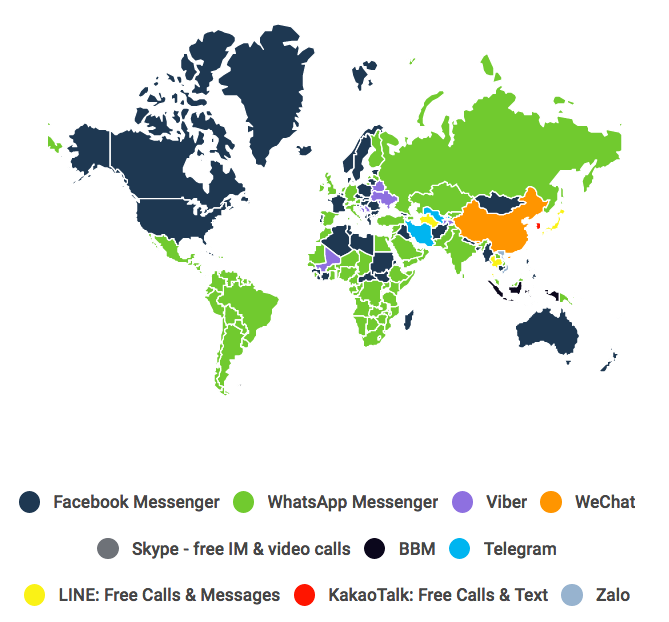
\includegraphics[width=0.7\textwidth]{images/similarweb-messenger-by-country.png}
	\caption{Most Popular Messaging App in Every Country~\cite{similarweb}}
	\label{fig:similarweb}
\end{figure}

\label{geography}

One important factor can be the geographical location of the target audience.
\\
As visible in figure \ref{fig:similarweb}, \emph{Facebook Messenger} and \emph{WhatsApp} are the global leading messengers,
and as previously mention the markets in China and Japan are dominated by \emph{WeChat} and \emph{Line} respectively,
but the data shows some lesser know trends; for example the \emph{Thai} market is also dominated by \emph{Line}
and in \emph{Iran}, \emph{Telegram} is the most popular messenger application.


\subsection{Cross-platform Development}
\label{crossplatform}

As with the creation of other kinds of software, it is possible to release the same chatbot software for multiple target platforms,
whereby the interaction between software and platform has to conform to the technical details and protocols of each environment, the usage of platform-specific features has to be adapted individually and the user experience needs to be designed to fit each environment's expectations.
\\

There are existing frameworks that allow developers to develop a chatbot once and release it to multiple platforms at the same time without any adjustments to individual platforms.
\\
One such framework is \emph{API.ai} by \emph{Google}.
As of writing it supports 16 different integrations, including platforms such as \emph{Facebook Messenger}, \emph{Skye} and \emph{Slack}~\cite{apiai}.
However, this platform is more than an adapter to different platforms.
It is complete solution to developing chatbots.
\emph{API.ai} comes with built-in support for natural language processing,
a chatbot is already able to have basic conversations out of the box,
and developers can train chatbots about new topics by just providing example conversations while the framework handles all of the language parsing.
\\
Detected keywords and intends can be forwarded to be handled with custom logic;
although for simple use cases this might not be necessary and a chatbot can be developed without writing a single line of code.
\\

Still, there are limits to platforms like \emph{API.ai}.
\\
First, intend parsing is, in the case if \emph{API.ai}, currently limited to a finite list of topics.
If a chatbot is handling topics from a domain unknown to \emph{API.ai}, this solution is not sufficient anymore.
\\
Further, developers have no control over the applied machine learning and natural language processing algorithms.
There are no possibilities for customization, if the parsing results or the generated responses do not match the requirements.
\\
Additionally, while \emph{API.ai} currently supports 15 different languages, a chatbot is limited to the available languages.
If a new language needs to be supported, a lot of work might be necessary switching to a custom solution.
\\
Another issue to keep in mind is, that, while \emph{API.ai} has support for many platform-specific features such as custom formats for message content and \emph{quick reply} buttons,
there are unique features of single platforms that are not supported
and since the space is evolving at such rapid pace future extentions might not be available either.
\\
As last point it should be mentioned that, even though \emph{API.ai} is at the moment free to use for everyone,
they will very likely search for a sustainable business model in the near future.
This business model could be simply charging for the service or collecting data which Google can use elsewhere, binding customers and gaining market share.
\\
Regardless which monetization strategy is chosen, as a developer one has to be aware that such a service is a non-controllable, external dependency.
